%%%%%%%%%%%%%%%%%%%%%%%%%%%%%%%%%%%%%%%%%%%%%%%%%%%%%%
% A Beamer template for University of Wollongong     %
% Based on THU beamer theme                          %
% Author: Qiuyu Lu                                   %
% Date: July 2024                                    %
% LPPL Licensed.                                     %
%%%%%%%%%%%%%%%%%%%%%%%%%%%%%%%%%%%%%%%%%%%%%%%%%%%%%%
% Customized for Sharif University of Technology     %
%%%%%%%%%%%%%%%%%%%%%%%%%%%%%%%%%%%%%%%%%%%%%%%%%%%%%%


\documentclass[serif, aspectratio=169]{beamer}
%\documentclass[serif]{beamer}  % for 4:3 ratio
\usepackage[T1]{fontenc} 
\usepackage{fourier} % see "http://faq.ktug.org/wiki/uploads/MathFonts.pdf" for other options
\usepackage{hyperref}
\usepackage{latexsym,amsmath,xcolor,multicol,booktabs,calligra}
\usepackage{graphicx,pstricks,listings,stackengine}
\usepackage{lipsum}

% For writing clean pseudocodes
\usepackage{algorithm, algpseudocode, mathtools, needspace}
% To justify the items
\usepackage{ragged2e}
% To draw diagrams
\usepackage{tikz}
% To include urls
\usepackage{url}
% To make clean tables
\usepackage{color, tabularray}

\author{Ali Sharifi-Zarchi}
\title{Machine Learning (CE 40717)}
\subtitle{Fall 2024}
\institute{
    CE Department \\
    Sharif University of Technology
}
\usepackage{SUTstyle}

% defs
\def\cmd#1{\texttt{\color{red}\footnotesize $\backslash$#1}}
\def\env#1{\texttt{\color{blue}\footnotesize #1}}
\definecolor{deepblue}{rgb}{0,0,0.5}
\definecolor{deepred}{RGB}{153,0,0}
\definecolor{deepgreen}{rgb}{0,0.5,0}
\definecolor{halfgray}{gray}{0.55}
\definecolor{silver}{rgb}{0.752,0.752,0.752}

\lstset{
    basicstyle=\ttfamily\small,
    keywordstyle=\bfseries\color{deepblue},
    emphstyle=\ttfamily\color{deepred},    % Custom highlighting style
    stringstyle=\color{deepgreen},
    numbers=left,
    numberstyle=\small\color{halfgray},
    rulesepcolor=\color{red!20!green!20!blue!20},
    frame=shadowbox,
}

% For writing comments that are aligned to the left side
\makeatletter
\NewDocumentCommand{\LeftComment}{s m}{%
  \Statex \IfBooleanF{#1}{\hspace*{\ALG@thistlm}}\(\triangleright\) #2}
\makeatother
% To manually indent states in algorithmicx
\newcommand{\IndState}{\State\hspace{\algorithmicindent}}
% To make breakable algorithms
\makeatletter
\newenvironment{nofloatalgorithmic}[2][0]
  {
  \par
  \needspace{\dimexpr\baselineskip+6.8pt}
  \noindent
  \hrule height.8pt depth0pt \kern2pt
  \refstepcounter{algorithm}
  \addcontentsline{loa}{algorithm}{\numberline{\thealgorithm}#2}
  \noindent\textbf{\fname@algorithm~\thealgorithm} #2\par
  \kern2pt\hrule\kern2pt
  \begin{algorithmic}[#1]
  }
  {
  \end{algorithmic}
  \nobreak\kern2pt\hrule\relax
  }
\makeatother
% To make vertical arrow
\newcommand\vertarrowbox[3][6ex]{%
  \begin{array}[t]{@{}c@{}} #2 \\
  \left\uparrow\vcenter{\hrule height #1}\right.\kern-\nulldelimiterspace\\
  \makebox[0pt]{\scriptsize#3}
  \end{array}%
}
% Clean argmin
\DeclareMathOperator*{\argmin}{arg\,min}

\begin{document}

\begin{frame}
    \titlepage
    \vspace*{-0.6cm}
    \begin{figure}[htpb]
        \begin{center}
            
\includegraphics[keepaspectratio, scale=0.25]{pic/sharif-main-logo.png}
        \end{center}
    \end{figure}
\end{frame}

\begin{frame}    
\tableofcontents[sectionstyle=show,
subsectionstyle=show/shaded/hide,
subsubsectionstyle=show/shaded/hide]
\end{frame}

\section{Unsupervised Learning Overview}
\begin{frame}{Unsupervised Learning}
    
    \begin{itemize}
        \item\textbf{Unsupervised Learning} involves analyzing unlabeled data to uncover hidden patterns or structures within the data
    \end{itemize}
\end{frame}

\begin{frame}{Some Common Tasks}
        \begin{itemize}
            \item \textbf{Clustering}: Grouping data points into clusters based on similarity.
            \item \textbf{Dimensionality Reduction}: Reducing the number of features under consideration and keeping (perhaps approximately) the most informative features.
            
        \item \textbf{Anomaly Detection}: Identifying data points that deviate significantly from the norm (e.g., fraud detection).

    \item \textbf{Generative Modeling}: Learning the distribution of data to generate new, similar instances.
        \end{itemize}
\end{frame}

\begin{frame}{Clustering}

        \begin{itemize}
        \item Clustering organizes data points into groups of similar objects.
\item Data points in a cluster are more similar to each other than to those in other clusters.
\item The notion of similarity depends on the task at hand (e.g., purchase behavior in market segmentation).
    \end{itemize}
\end{frame}

\begin{frame}{Some Applications of Clustering}
\begin{itemize}
    \item Customer Segmentation (Marketing)
    \item Image Segmentation and Object Detection (Computer Vision)
    \item Anomaly Detection (Cybersecurity, Finance)
    \item Genomics and Bioinformatics
    \item Social Network Analysis and Community Detection
\end{itemize}
\end{frame}


\begin{frame}{Clustering in Action: Music Recommendation Systems }
\begin{itemize}
    \item Music recommendation systems cluster songs based on similarity.
    % \item Fun little exercise to build a simple system at \href{https://machinelearninggeek.com/spotify-song-recommender-system-in-python/}{machinelearninggeek.com}, after finishing this chapter.
\end{itemize}
  
    \begin{figure}
        \centering
        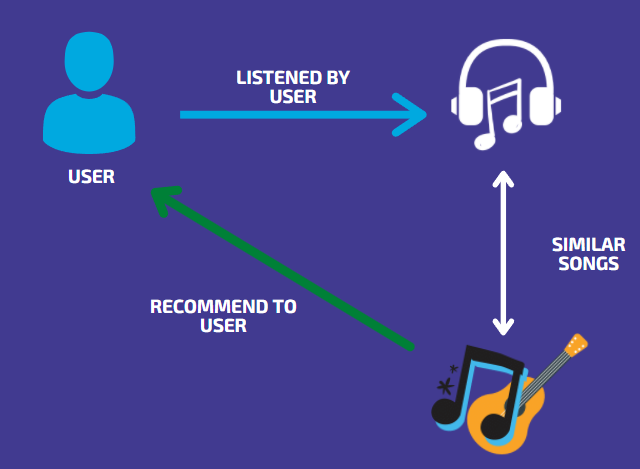
\includegraphics[scale=0.3]{pic/figs/image-4.png}
        {\scriptsize Adopted from \href{https://machinelearninggeek.com/spotify-song-recommender-system-in-python/}{machinelearninggeek.com}}
        
    \end{figure}
\end{frame}


\begin{frame}{Clustering in Action: Music Recommendation Systems }
\begin{itemize}
    \item When you like a song, the system suggests others from the same cluster.
    
\end{itemize}

    \begin{figure}
        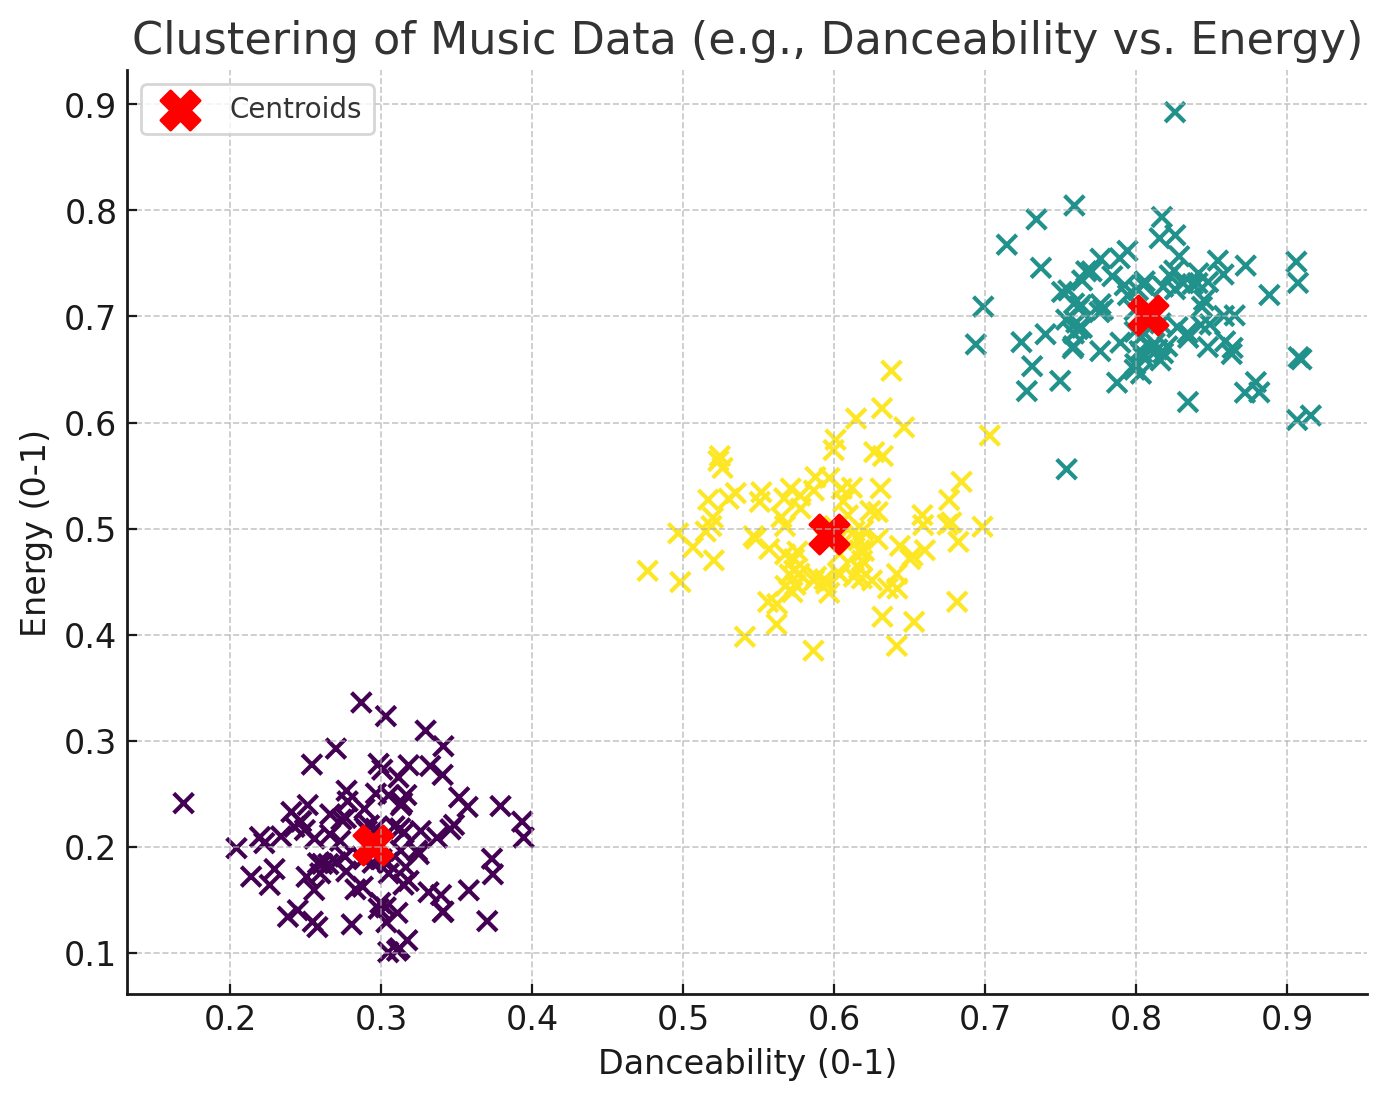
\includegraphics[scale=0.4]{pic/figs/Music Clustering2.png}
        \centering
    \end{figure}

        
\end{frame}

\begin{frame}{Clustering in Action: Gene Expression Clustering}
\begin{itemize}
    \item Clustering can decipher hidden patterns in gene expression data, which can help in understanding disease mechanisms or genetic variations.
\end{itemize}
    \begin{figure}
        \centering
        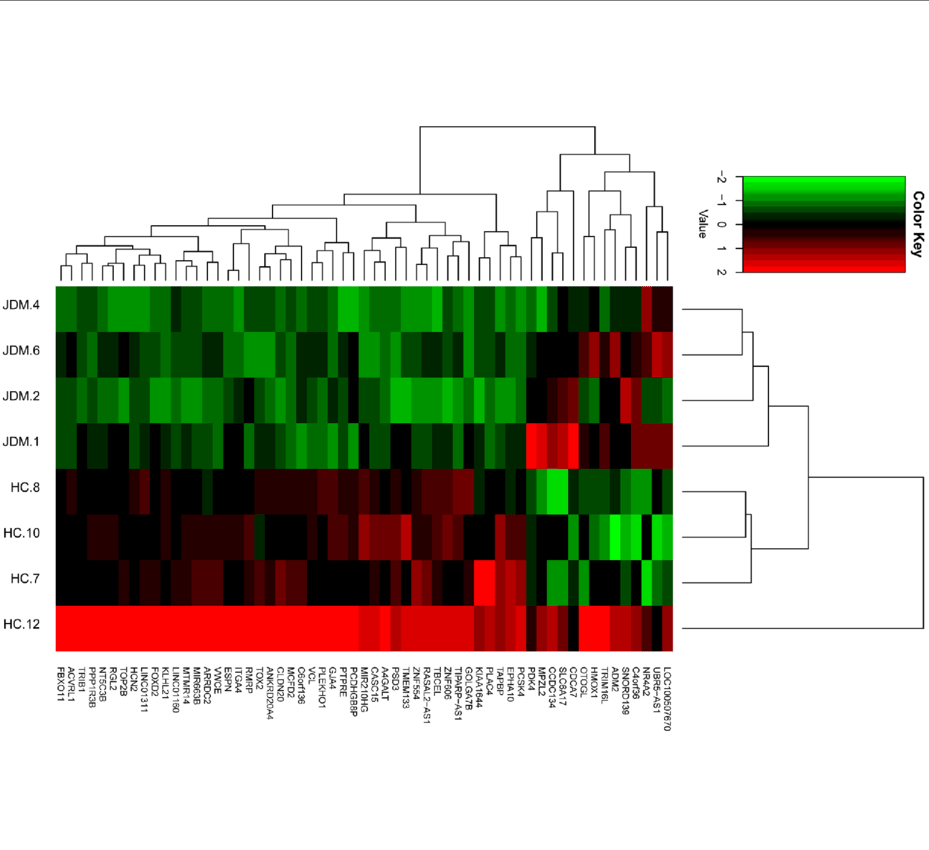
\includegraphics[scale=0.35]{pic/figs/Unsupervised-hierarchical-clustering-analysis-of-gene-expression.png}
         {\scriptsize Adopted from \href{https://www.researchgate.net/publication/334433467_Plasma_exosomes_from_children_with_juvenile_dermatomyositis_are_taken_up_by_human_aortic_endothelial_cells_and_are_associated_with_altered_gene_expression_in_those_cells}{www.researchgate.net}}
        
    \end{figure}
    
\end{frame}

\begin{frame}{Two Beginning Questions}
    \begin{itemize}

\item How to create 'good' clusters?
\item How many clusters do we need?

    \end{itemize}
\end{frame}


% \begin{frame}{Analysing the task}
% \begin{itemize}

%     \item Usually two general ways to measure similarity:
%     \begin{itemize}
%         \item A similarity function $s(x_i,x_j)$ that is larger when $x_i$ and $x_j$ are more similar. like cosine similarity.
%         \item A dissimilarity or distance function $d(x_i,x_j)$ that is smaller the more simialr to points are. like euclidean distance.
%     \end{itemize}
%     \item Each algorithm might require extra properties
%             % \item Extra Note: Most algorithms require a distance function to be a \textbf{proper metric} and the similarity measure to create a \textbf{PSD matrix} for all pairs of a finite number of data points.
            
% \end{itemize}
% \end{frame}

\section{K-Means}
\begin{frame}{K-Means overview}
    \begin{itemize}
        \item The most widely used clustering algorithm.
        \item Partitions data into $K$ distinct groups based on feature similarity
        \item It works by \textbf{iteratively} assigning data points to the nearest centroid (mean of the group) and then recalculating the centroids based on the new group memberships
        \item The process repeats until the assignments no longer change
    \end{itemize}
\end{frame}

% \begin{frame}{K-Means overview}
%     \begin{itemize}
%       \item K-Means assumes we know there are $K$ clusters, or we want $K$ clusters.
%         \item It works by \textbf{iteratively} assigning data points to the nearest centroid (mean of the group) and then recalculating the centroids based on the new group memberships
%         \item The process repeats until the assignments no longer change
%     \end{itemize}
% \end{frame}


% K means in action
\begin{frame}{K-Means in action}
    \begin{figure}
        \centering
        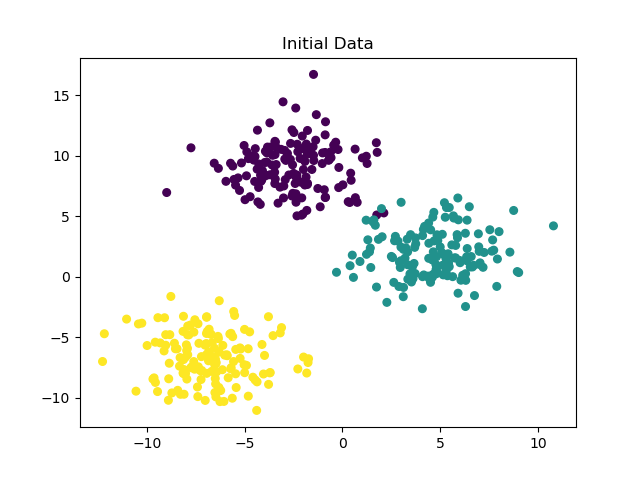
\includegraphics[width=\textwidth]{kmeans_in_action_figures/original.png}
    \end{figure}
\end{frame}

\begin{frame}{K-Means in action}
    \begin{figure}
        \centering
        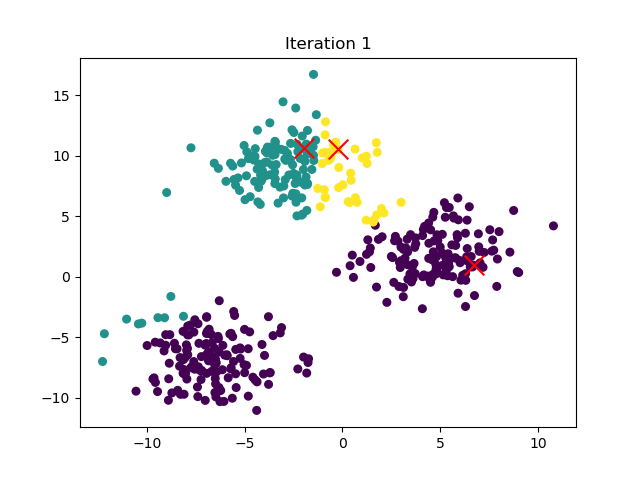
\includegraphics[width=\textwidth]{kmeans_in_action_figures/kmeans_iter_1.png}
    \end{figure}
\end{frame}
\begin{frame}{K-Means in action (cont.)}
    \begin{figure}
        \centering
        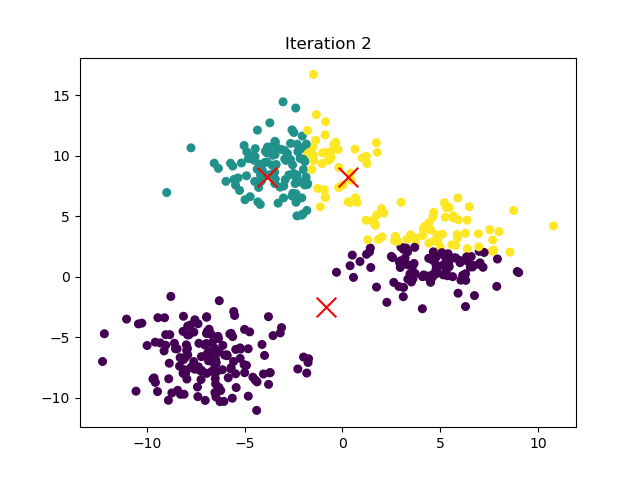
\includegraphics[width=\textwidth]{kmeans_in_action_figures/kmeans_iter_2.png}
    \end{figure}
\end{frame}

\begin{frame}{K-Means in action (cont.)}
    \begin{figure}
        \centering
        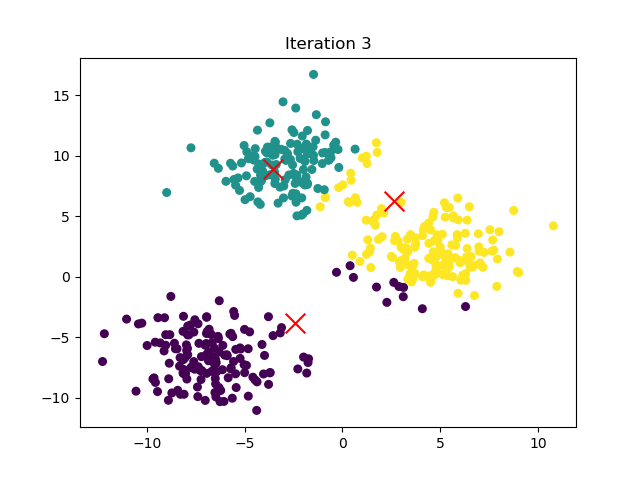
\includegraphics[width=\textwidth]{kmeans_in_action_figures/kmeans_iter_3.png}
    \end{figure}
\end{frame}
\begin{frame}{K-Means in action (cont.)}
    \begin{figure}
        \centering
        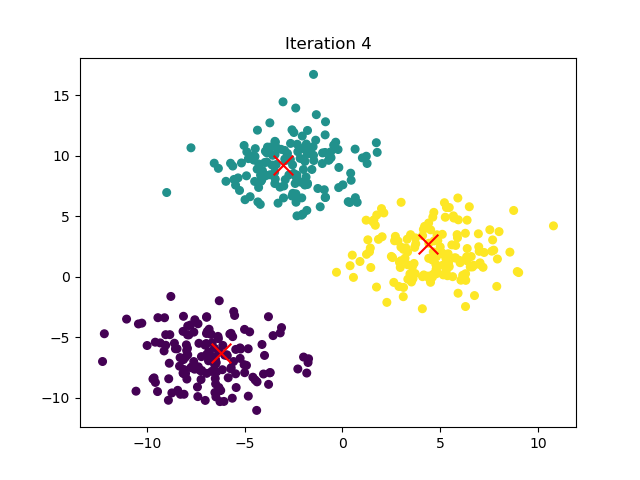
\includegraphics[width=\textwidth]{kmeans_in_action_figures/kmeans_iter_4.png}
    \end{figure}
\end{frame}
\begin{frame}{K-Means in action (cont.)}
    \begin{figure}
        \centering
        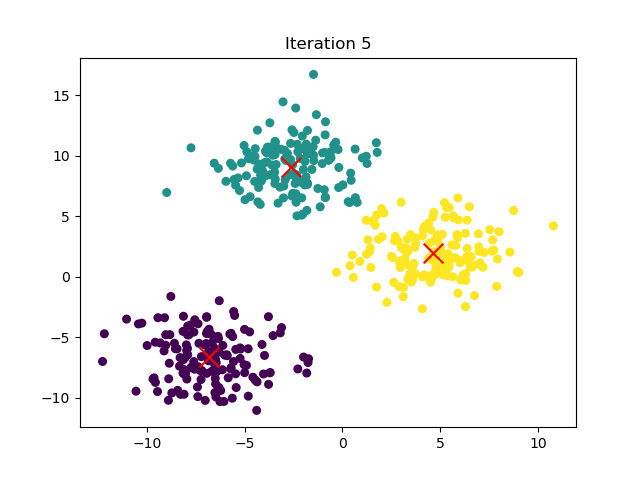
\includegraphics[width=\textwidth]{kmeans_in_action_figures/kmeans_iter_5.png}
    \end{figure}
\end{frame}

\begin{frame}{Algorithm}
    \begin{algorithm}[H]
    \caption{K-means Clustering}\label{alg:KMeans}
    \begin{algorithmic}[1]
        \State \textbf{Input:} $K$ (number of clusters), $D = \{\boldsymbol{x}^{(1)}, \dots, \boldsymbol{x}^{(N)}\}$ (data points)
        \State \textbf{Initialize:} Select $K$ random points as centroids $\{\boldsymbol{\mu}_1, \dots, \boldsymbol{\mu}_K\}$

        \Repeat
            \State
            \For{each $1\leq i \leq N$}
            Assign each point $\boldsymbol{x}^{(i)}$ to nearest centroid $f(\boldsymbol{x}^{(i)} ) = \arg \min_{j} \|\boldsymbol{x}^{(i)} - \boldsymbol{\mu}_j\|$
            \State \EndFor
            \State \For{each $1\leq j \leq K$}
             \State set $C_j = \{x^{(i)}|f(x^{(i)})=j\}$
             \State Update centroids $\boldsymbol{\mu}_j = \frac{1}{|C_j|} 
             \sum_{\boldsymbol{x}^{(i)} \in C_j} \boldsymbol{x}^{(i)}$
             \State \EndFor
        \Until{Centroids do not change}
    
        \State \textbf{Output:} Final clusters $\{C_1, C_2, \dots, C_K\}$
    \end{algorithmic}
    \end{algorithm}
\end{frame}

\begin{frame}{Problem definition}
    \begin{itemize}
        \item Formally: We have $X_{\text{train}} = \{ x^{(1)}, x^{(2)}, \dots, x^{(N)} \} \subseteq \mathbb{R}^d$
        \item $K$ is the number of clusters.
        \item We are learning:
        \begin{enumerate}
            \item A function or mapping $f:\mathbb{R}^d\to \{1,2, \dots , K\}$ that assigns a cluster to each data point.
            \item A set of \( K \) prototypes \(\mu = \{ \mu_1, \mu_2, \dots, \mu_K  \} \subseteq \mathbb{R}^d \) as the cluster representatives, called \textbf{centeroids}.
        \end{enumerate}
       
    \end{itemize}
\end{frame}

\begin{frame}{Objective Function}
\begin{itemize}

    \item We want samples in the same cluster to be similar.
    \item In K-Means, this is expressed as:

    $$
    J = \sum_{j=1}^K \sum_{x^{(i)}\in C_j} || x^{(i)} -  \mu_j ||^2
    $$

\item Choose $f$ and $\mu = \{\mu_1,\mu_2,\dots,\mu_K\}$ to minimize this.
        \item This problem is NP-hard. K-Means is a heuristic solution, which is NOT guaranteed to find optimal solution.
\end{itemize}
\end{frame}


\begin{frame}{K-Means Process Example}

\begin{figure}
        \centering
        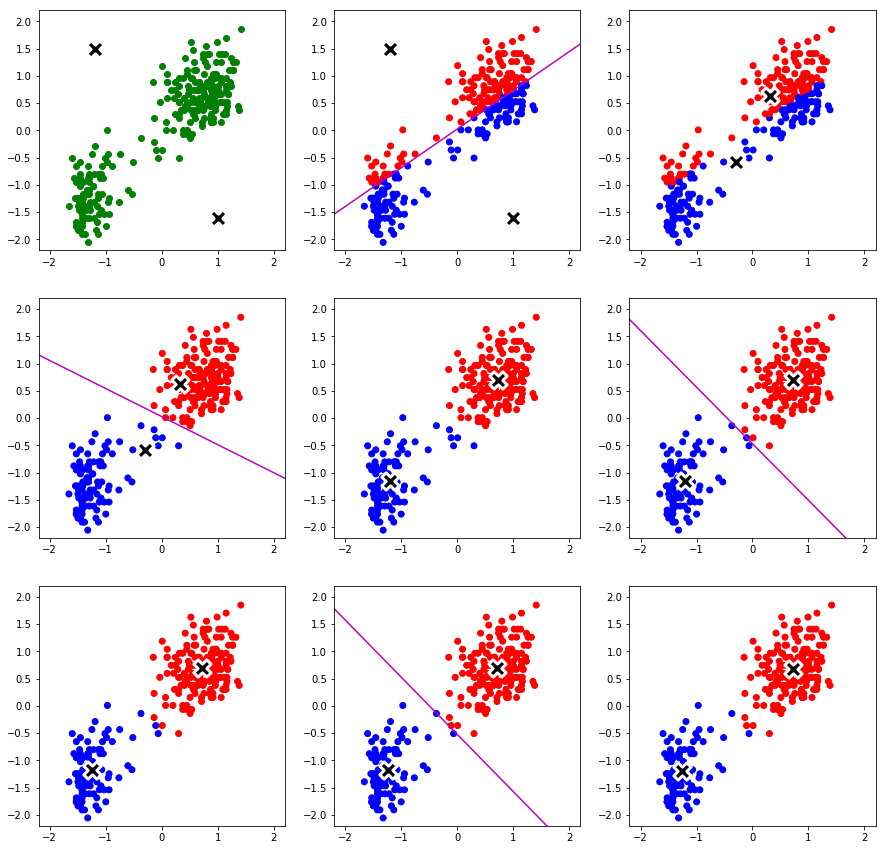
\includegraphics[width=\textwidth]{pic/figs/Clustering_K-means_7_1.png}
        {\scriptsize Adopted from \href{https://mlbhanuyerra.github.io/2018-02-19-Clustering-K-means/}{mlbhanuyerra.github.io}}
    \end{figure}
\end{frame}


\begin{frame}{Convergence}
    \begin{itemize}
    \item How do we know K-Means will converge in a finite number of steps ?
    \item First we show in each step $J$ will decrease, as long as we have not converged.
    \end{itemize}
\end{frame}

\begin{frame}{Convergence (cont.)}
\begin{itemize}
\item We initially assigne each sample to the nearest centroid.
$$ f(x) : = \textit{argmin}_j \; ||x - \mu_j||^2 $$.

\item Keep each sample's assignment fixed until a closer centriod is found.
\item Each time a sample is reassigned. the total distance between samples and their centroids decreases.
\item The number of possible sample-to-centroid assignments is finite.

\item The algorithm terminates when no sample changes its assigned centroid.
            
\end{itemize}
    
\end{frame}

\begin{frame}{Convergence (cont.)}
\begin{itemize}
    \item In Updating step, with $f(x)$ fixed, $J$ is a quadratic function of $\mu_j$ (like SSE) and by taking derivative we can minimize it as:
    $$
        \frac{\partial J}{\partial \mu_j } = 0 \implies \sum_{x^{(i)} \in C_j} 2 \left(x^{(i)} - \mu_j \right) = 0
    $$
    \item This means we should \textbf{update} each $\mu_j$ as the mean of cluster $C_j$:
    $$
        \mu_j = \frac{\sum_{x^{(i)} \in C_j} x^{(i)}}{|C_j|}
    $$
\end{itemize}
\end{frame}

\begin{frame}{Convergence (cont.)}
    \begin{itemize}
        \item For each cluster, the mean of its samples minimizes squared distances.
        \item For $C_j$ if $\mu'_j$ was the old centroid we have: $\sum_{x^{(i)} \in C_j} ||x^{(i)}-\mu'_j||^2 \geq \sum_{x^{(i)} \in C_j} ||x^{(i)}-\mu_j||$. So  $J_{\text{new}} \leq J_{\text{old}} $.
    \end{itemize}
\end{frame}

\begin{frame}{Convergence (cont.)}
    \begin{itemize}
\item $J$ is non-negative, and there are a finite number of partitions so there is a minimum for $J$ and we can't decrease $J$ forever.
 \item  Therefore we must converge at some point.
\item  The convergence properties of the K-means algorithm were studied by MacQueen (1967).

    \end{itemize}
\end{frame}

\begin{frame}{K-Means Convergence (cont.)}
    \begin{figure}
        \centering
        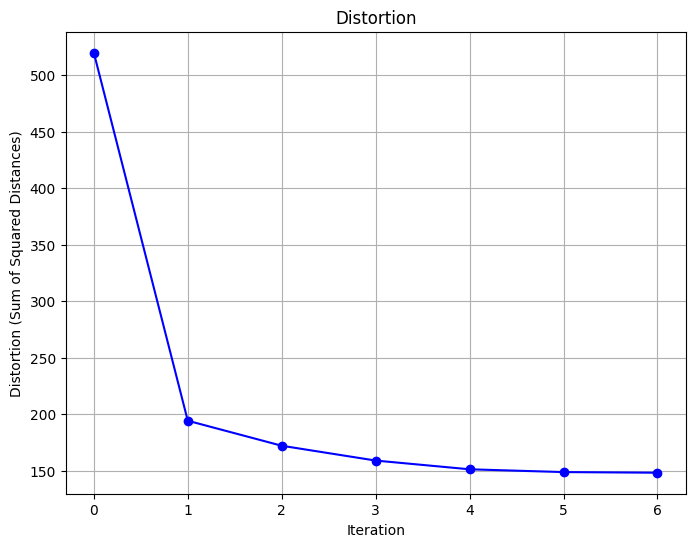
\includegraphics[scale=0.45]{pic/figs/distortion.png}
        
    \end{figure}
\end{frame}

% \begin{frame}{Optional Adventure}
%     \item  Each Assignment and Updating step in K-Means corresponds respectively to the E (expectation) and M (maximization) steps of the EM algorithm.
%     \item One can prove that k-means is equivalent to running EM on a particular Naive Bayes Model.  
% \end{frame}

\begin{frame}{Strengths}
    \begin{itemize}
        \item Simple: easy to understand and to implement.
        \item  Efficient: Time complexity: $O(tkn)$, 
where
\begin{itemize}
    
\item  $n$ is the number of data points, 
\item $k$ is the number of clusters, and 
\item $t$ is the number of iterations. 
\end{itemize}
% – Since both k and t are usually small. k-means is considered a linear algorithm. (personally not sure about this ???)
        
    \end{itemize}
\end{frame}

\section{Challenges in K-Means}


\begin{frame}{Initialization}
    \begin{itemize}
    
        \item K-Means always converges. What could go wrong ?
        \item K-Means algorithm is a \textbf{heuristic}
        \item It requires initial centroids, and
the choice is important as it could
affect the $t$ in $O(tkn)$.

    \end{itemize}
\end{frame}

\begin{frame}{Local Optimum}
    \begin{itemize}
        \item The algorithm finds a local minimum but there is no guarantee to find global minimum.
        \item Its result is highly affected by the initialization.
        \item Some suggestions are:
        \begin{itemize}
            \item  Multiple runs with random initial centroids, then select the "best" result.
            \item Initialization heuristics (K-Means++ , Furthest Traversal).
            \item Initializing with the suggested results of another method.
        \end{itemize}
    \end{itemize}
\end{frame}

\begin{frame}{Local Optimum}
 
        \begin{figure}
            \centering
            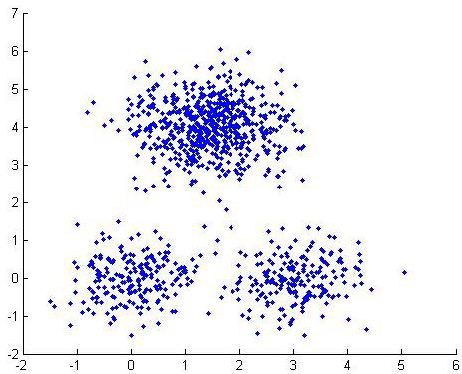
\includegraphics[scale=0.55]{pic/original_data.png}
        \end{figure}
    =
\end{frame}

\begin{frame}{Local optimum (cont.)}
    \begin{minipage}{0.5\textwidth}
        \begin{figure}
            \centering
            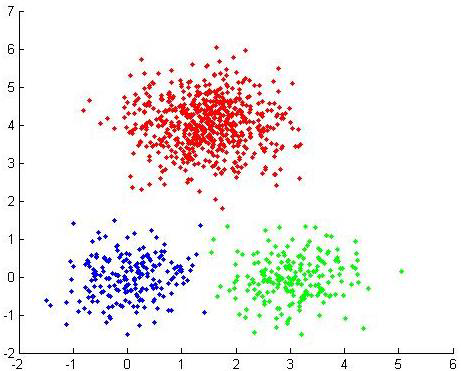
\includegraphics[scale=0.55]{pic/optimal_clustering.png}
        \end{figure}
        \vfill
        \begin{center}
            Optimal clustering
        \end{center}
    \end{minipage}%
    \begin{minipage}{0.5\textwidth}
        \begin{figure}
            \centering
            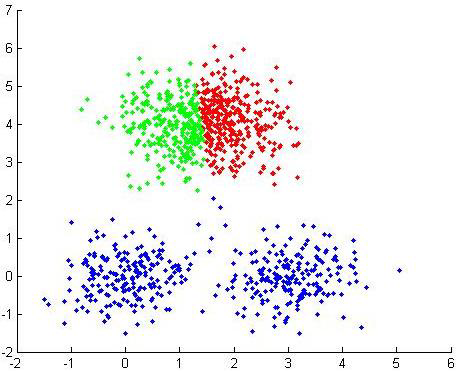
\includegraphics[scale=0.55]{pic/possible_clustering.png}
        \end{figure}
        \vfill
        \begin{center}
            Possible clustering
        \end{center}
    \end{minipage}
\end{frame}


\begin{frame}{Definition of Mean}
    \begin{itemize}
        \item We assume $x^{(i)} \in \mathbb{R}^d$, which is not always the case. K-Means requires a space where sample \textbf{mean} is defined.
        \begin{itemize}
            \item Categorical data. 
            \item  A suggested solution: K-Mode - the centroid is the most frequent category (the mode) in each cluster.
            \item Closest centroid is found by the Hamming Distance.
        \end{itemize}


    \end{itemize}
\end{frame}

\begin{frame}{How many clusters?}
    \begin{figure}
        \centering
        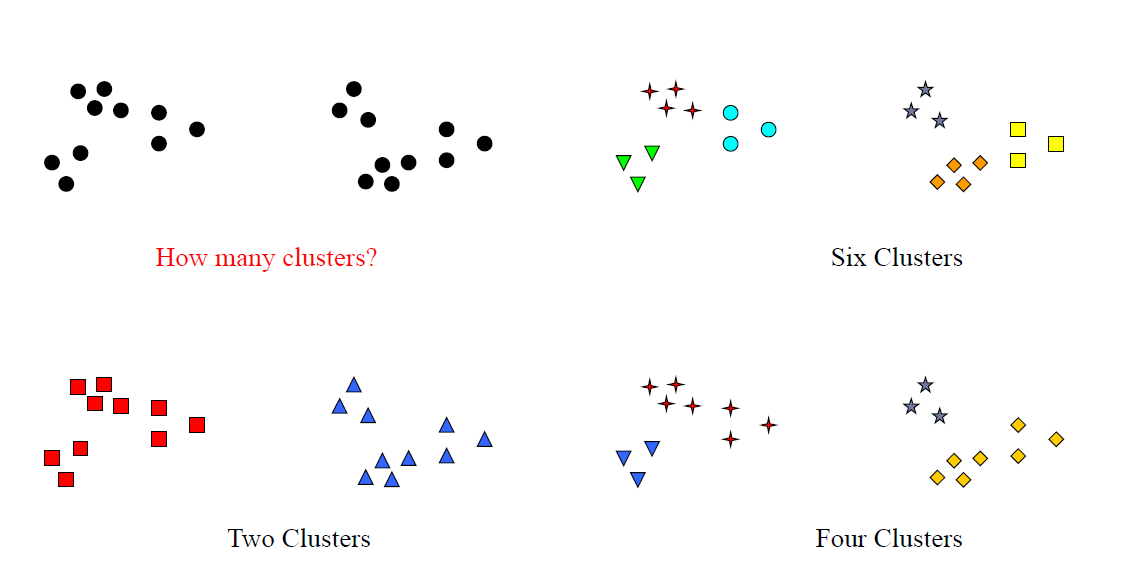
\includegraphics[scale=0.5]{pic/how_many_clusters.png}
        {\scriptsize Adopted from slides of Dr. Soleymani, Modern Information Retrieval Course, Sharif University of technology.}
    \end{figure}
\end{frame}


\begin{frame}{How many clusters? (cont.)}
    \begin{itemize}
        \item Number of clusters is usually given in advance in the problem of clustering. However; finding the right number of clusters is also a problem.
        \item First we need to know how we can evaluate a clustering.
    \end{itemize}
\end{frame}


\begin{frame}{Clustering Evaluation}
    \begin{itemize}
        \item Evaluating clusters involves two key aspects:
        \begin{itemize}
            \item \textbf{Intra-cluster cohesion (compactness)}: How similar the data points are within a cluster.
            \item Often measured by the within-cluster sum of squares (WCSS):
            $$
            WCSS = \sum_{i=1}^K \sum_{x \in C_i} ||x-\mu_i||^2
            $$
        \end{itemize}
    \end{itemize}
\end{frame}


\begin{frame}{Clustering Evaluation}
    \begin{itemize}
        \item \textbf{Inter-cluster separation (isolation)}: How different the data points are between clusters.
        
        \begin{itemize}
          \item Single-link (Minimum Distance):
            \item Measures the **minimum distance** between any two points from different clusters.

            \[
            d_{\text{single}}(C_i, C_j) = \min_{x \in C_i, y \in C_j} d(x, y)
            \]
        
        \item Complete-link (Maximum Distance):
            \item Measures the maximum distance between any two points from different clusters.
            \[
            d_{\text{complete}}(C_i, C_j) = \max_{x \in C_i, y \in C_j} d(x, y)
            \]
        \end{itemize}
    \end{itemize}
\end{frame}

\begin{frame}{Clustering Evaluation}
    \begin{itemize}
    \item \textbf{Inter-cluster separation (isolation)}: How different the data points are between clusters.
        \begin{itemize}
        \item Centroid (Ward’s Method):
            \item Measures the distance between the centroids of two clusters.
            \[
            d_{\text{centroid}}(C_i, C_j) = d(\mu_i, \mu_j)
            \]
    
        \item Average-link:
            \item Measures the average distance between all pairs of points from different clusters.
            \[
            d_{\text{average}}(C_i, C_j) = \frac{1}{|C_i| \cdot |C_j|} \sum_{x \in C_i} \sum_{y \in C_j} d(x, y)
            \]
        \end{itemize}
    \end{itemize}
\end{frame}


\begin{frame}{Elbow Method for Optimal K}
    \begin{itemize}
        \item Finds the optimal number of clusters $K$ by minimizing the within-cluster sum of squares (WCSS).
        \item Elbow Point:
        \begin{itemize}
            \item Plot WCSS versus $K$.
            \item The point where the rate of decrease sharply slows down (resembles an "elbow") is considered the optimal $K$.
        \end{itemize}
    \end{itemize}
    \begin{figure}
        \centering
        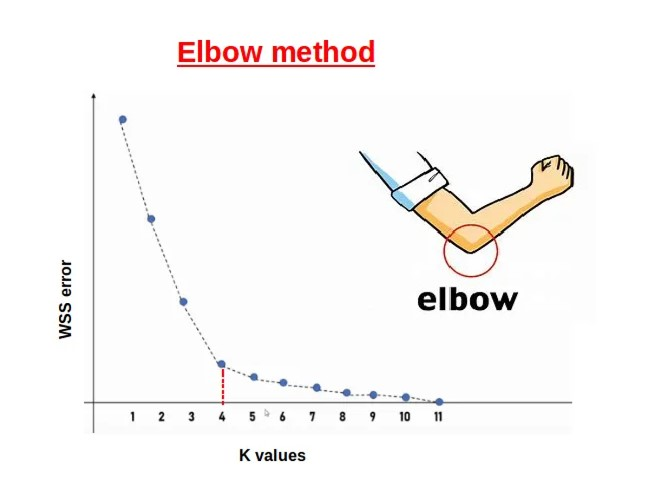
\includegraphics[scale = 0.45]{pic/figs/elbow.jpg}
         {\scriptsize Adopted from  \href{https://medium.com/@zalarushirajsinh07/the-elbow-method-finding-the-optimal-number-of-clusters-d297f5aeb189}{medium.com}}
        
        \label{fig:my_label}
    \end{figure}
\end{frame}

\begin{frame}{Silhouette Method for Cluster Evaluation}
    \begin{itemize}
        \item Silhouette Score for a single point $i$:
        $$
        S(i) = \frac{b(i)-a(i)}{max(a(i),b(i))}
        $$
        \item where:
        \begin{itemize}
            \item  $a(i)$ is the average distance between $i$ and all other points in the same cluster.
            \item $b(i)$ is the average distance between $i$ and points in the nearest neighboring cluster.
        \end{itemize}
        \item Interpretation:
\begin{itemize}
    \item $ S(i) \in [-1, 1]$
    \item $ S(i) \approx 1$ : Well-clustered.
    \item  $S(i) \approx 0$ : On or near the decision boundary between clusters.
    \item  $S(i) \approx -1$ : Misclustered.
\end{itemize}
    \end{itemize}
\end{frame}

\begin{frame}{How many Clusters? (cont.)}
\begin{itemize}
    \item There is a trade-off between having better focus within each cluster or having too many clusters.
        \item  Don't want one-element clusters.
        \item \textbf{Optimization problem:} penalize having too many clusters
        \[
        K^* = \ arg \ min_k \  J(k) + \lambda k 
        \]
\end{itemize}
    
\end{frame}

\begin{frame}{Outliers}
        \begin{itemize}
    \item The algorithm is sensitive to outliers
            \item Outliers are data points that are very far away from other data points. 
\item Outliers could be errors in data
recording or unique data points
with significantly different
values.
% \item K-medoids  and DBSCAN are more robust to outliers.
        \end{itemize}
\end{frame}

\begin{frame}{Data Distribution}
    \begin{itemize}
        \item There is a problems with how k-means defines clusters.
        \item  K-means assumes clusters are spherical and separated by equal variance, which limits its effectiveness on non-spherical or complex-shaped clusters.
    \begin{figure}
        \centering
        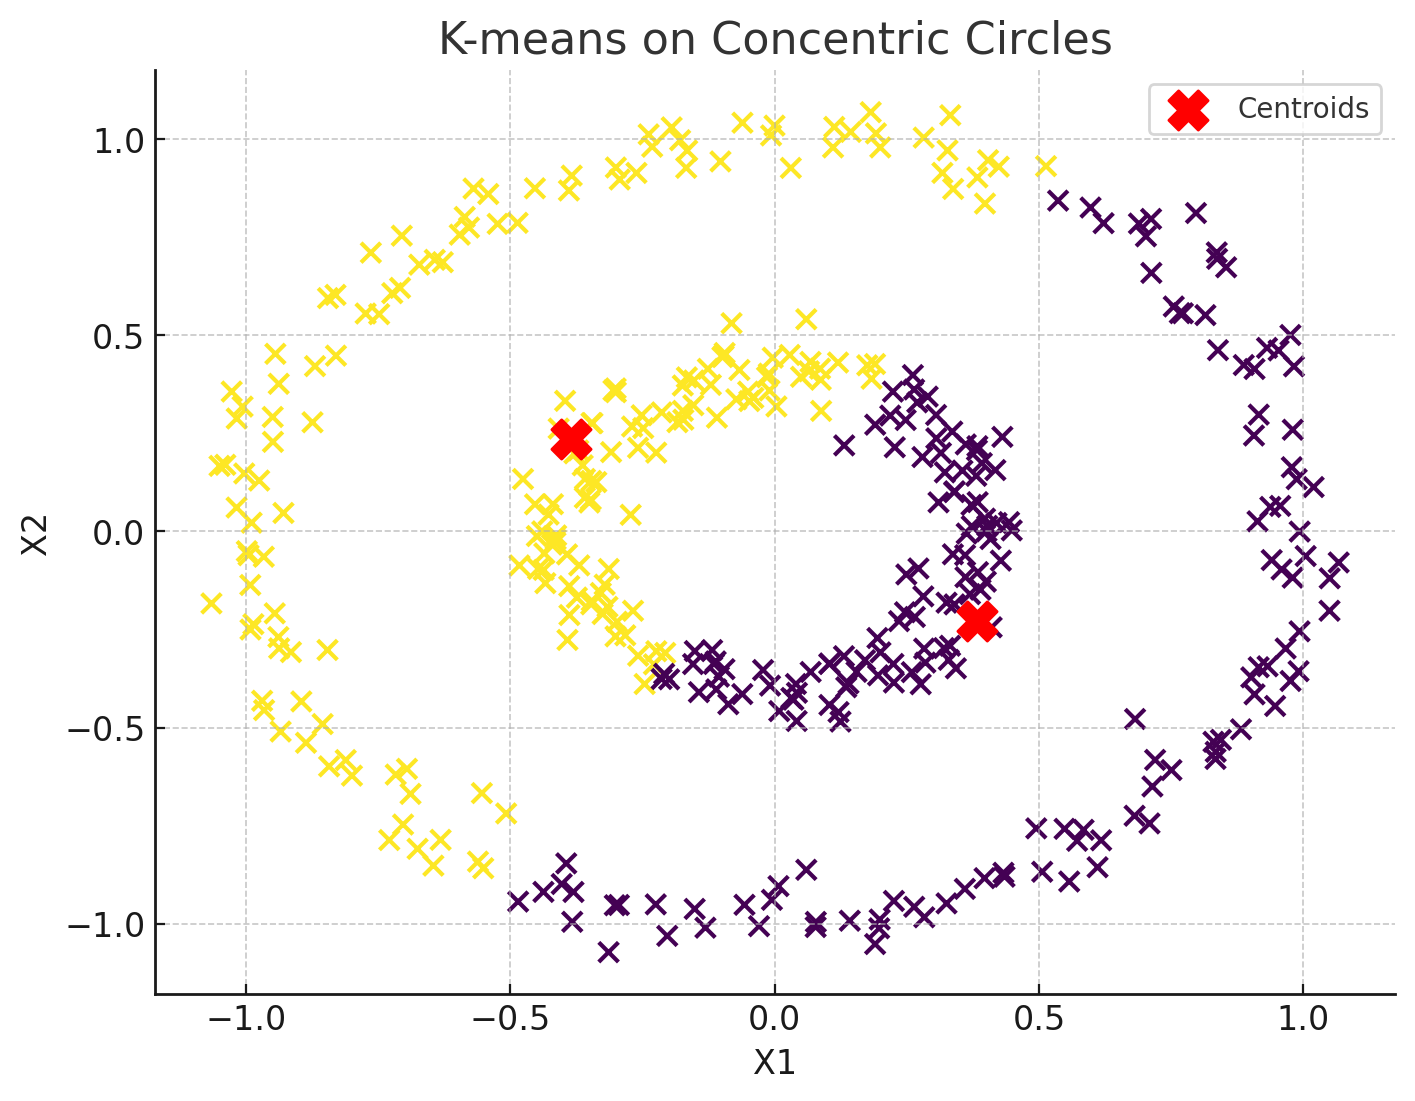
\includegraphics[scale=0.35]{pic/figs/kmeans_anti.png}
        \caption{example when k-means wont work}
    \end{figure}

    \end{itemize}
\end{frame}


\section{Other Clustering Algorithms}

\begin{frame}{Hard vs Soft Clustering}
    \begin{minipage}{0.55\textwidth}
        \begin{itemize}
        \item \textbf{Hard Clustering(Partitional)}: Each data point belongs to exactly one cluster
        \begin{itemize}
            \item More common and easier to use.
        \end{itemize}
        \item \textbf{Soft Clustering(Bayesian)}
    \end{itemize}
    \end{minipage}%
    \begin{minipage}{0.40\textwidth}
        \begin{figure}
            \centering
            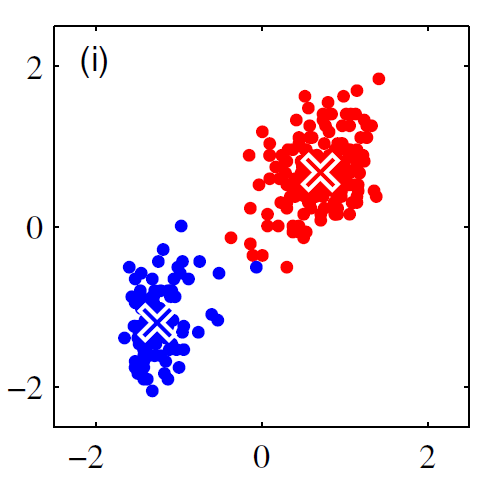
\includegraphics[scale=0.5]{pic/hard_clustering.png}
            {\scriptsize Figure adapted from Machine Learning and Pattern Recognition, Bishop}
        \end{figure}
    \end{minipage}
    
\end{frame}

\begin{frame}{Hard vs Soft Clustering (cont.)}
    \begin{minipage}{0.55\textwidth}
        \begin{itemize}
        \item \textbf{Hard Clustering(Partitional)}
        \item \textbf{Soft Clustering(Bayesian)}: Each sample is assigned to different clusters with probabilities, rather than $\{0,1\}$.
        \begin{itemize}
            \item data point belongs to each cluster with a probability
        \end{itemize}
        
    \end{itemize}
    \end{minipage}%
    \begin{minipage}{0.40\textwidth}
        \begin{figure}
            \centering
            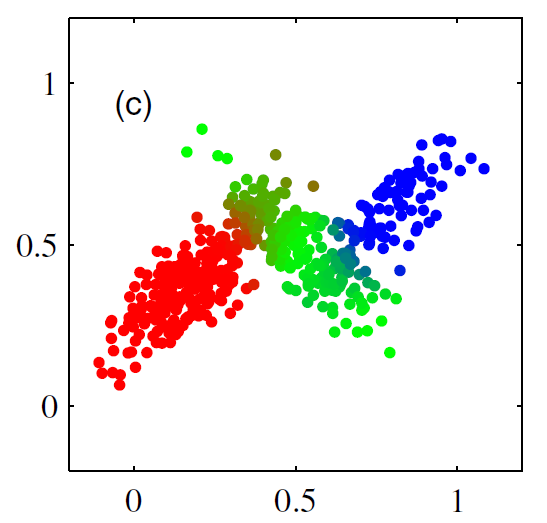
\includegraphics[scale=0.5]{pic/soft_clustering.png}
            {\scriptsize Figure adapted from Machine Learning and Pattern Recognition, Bishop}
        \end{figure}
        
    \end{minipage}
    
\end{frame}


% \begin{frame}{Hierarchical Algorithms}
% \begin{itemize}
%     \item The Traditional algorithms for clustering are usually categorized as: 
%     \begin{itemize}
%         \item \textbf{ Hierarchical} algorithms find successive clusters using previously established clusters. Two types:
% \begin{itemize}
% \item \textit{ Agglomerative } algorithms begin
% with each element as a separate
% cluster.
%     \item \textit{ Divisive } algorithms begin with the
% entire set as a single cluster.
% \end{itemize}
%     \end{itemize}
% \end{itemize}
% \end{frame}

\begin{frame}{Hierarchical Clustering}
    
    \begin{itemize}
    \item \textbf{ Hierarchical} algorithms find successive clusters using previously established clusters. Two Types:
        \begin{itemize}
            
        \item \textbf{Agglomerative (bottom-up)}: Start with individual points and merge clusters.
        \item \textbf{Divisive (top-down)}: Start with all points and split clusters.
        \end{itemize}
    \textbf{Result:} A hierarchy of clusters represented by a dendrogram.
    \end{itemize}
    \begin{figure}
        \centering
        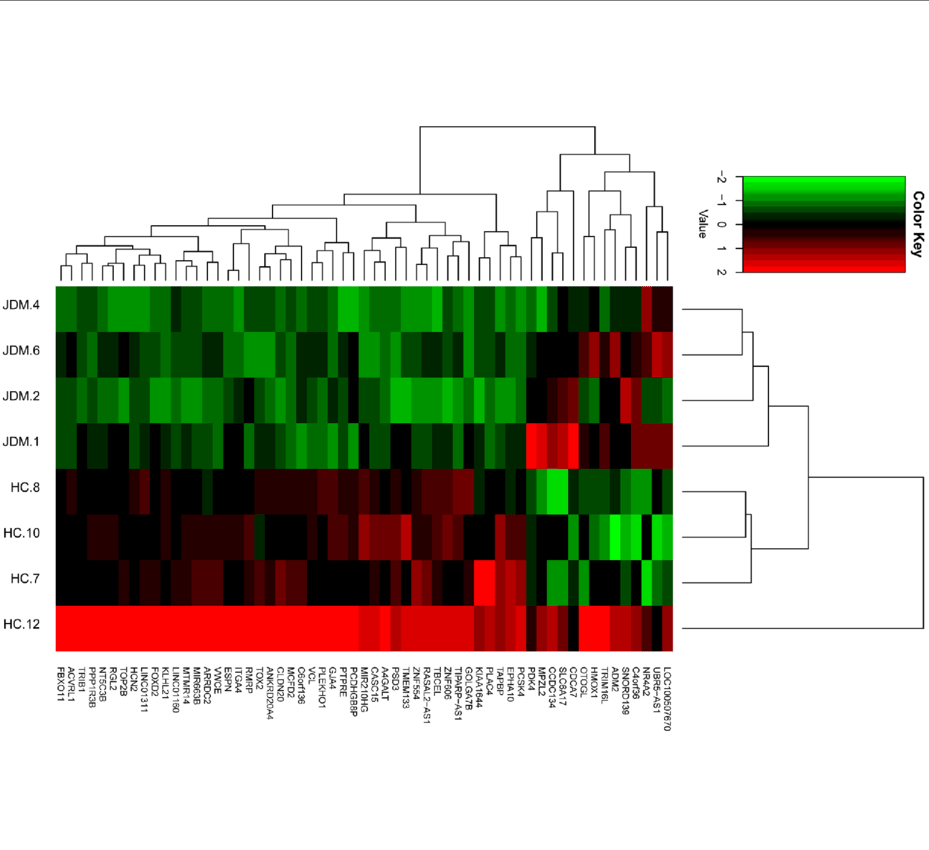
\includegraphics[scale=0.30]{pic/figs/Unsupervised-hierarchical-clustering-analysis-of-gene-expression.png}
        \caption{Figure from \href{https://www.researchgate.net/publication/334433467_Plasma_exosomes_from_children_with_juvenile_dermatomyositis_are_taken_up_by_human_aortic_endothelial_cells_and_are_associated_with_altered_gene_expression_in_those_cells}{www.researchgate.net}}
    \end{figure}
\end{frame}

\begin{frame}{Agglomerative Clustering Algorithm}
    \begin{itemize}
        \item Start with each point as its own cluster.
        \item Merge the "closest" clusters.
        \item Repeat until one cluster remains or desired number is reached.
        \item Closest cluster can be determined using inter-cluster separation measures
    \end{itemize}
\end{frame}

\begin{frame}{Dendrogram and Cutting}
    \begin{itemize}
        \item A dendrogram shows the hierarchy of merges.
        \item Cut the dendrogram at a desired level to form clusters.
    \end{itemize}
    \begin{figure}
        \centering
        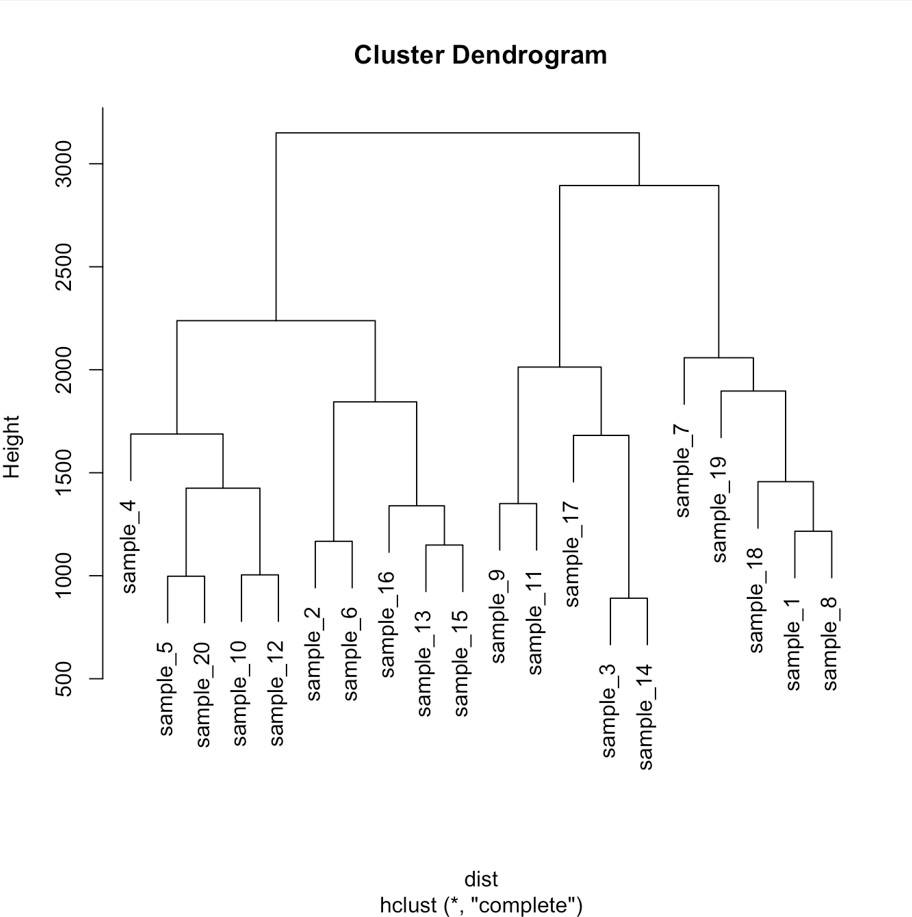
\includegraphics[scale=0.30]{pic/figs/dendrogram.jpg}
        {\scriptsize Adopted from \href{https://r-graph-gallery.com/29-basic-dendrogram.html}{r-graph-gallery.com}}
       
        \label{fig:dendrogram}
    \end{figure}
\end{frame}

\begin{frame}{Hierarchical Algorithms}
\begin{itemize}
    \item Advantages:
     \begin{itemize}
        \item No need to specify the number of clusters.
        \item Produces a dendrogram for visualization.
        \item Works with arbitrary-shaped clusters.
    \end{itemize}
    \item Disadvantages
    \begin{itemize}
        \item High computational cost.
        \item Sensitive to noise and outliers.
        \item Greedy: cannot undo merges.
    \end{itemize}
\end{itemize}
   
\end{frame}


\begin{frame}{DBSCAN}
    \textbf{DBSCAN (Density-Based Spatial Clustering of Applications with Noise):}
    \begin{itemize}
        \item Groups points in high-density regions.
        \item Labels points in low-density regions as noise.
        \item Does not require specifying the number of clusters $K$.
    \end{itemize}
    
    \textbf{Parameters:}
    \begin{itemize}
        \item $ \epsilon $ (epsilon): Maximum distance for neighbors.
        \item \texttt{minPts}: Minimum points to form a dense region.
    \end{itemize}
\end{frame}

\begin{frame}{Core Concepts in DBSCAN}
    \textbf{DBSCAN defines three types of points:}
    \begin{itemize}
        \item \textbf{Core Point}: A point with at least \texttt{minPts} neighbors within distance $ \epsilon $.
        \item \textbf{Border Point}: A point within $ \epsilon $ of a core point but with fewer than \texttt{minPts} neighbors.
        \item \textbf{Noise}: Points that are neither core points nor border points.
    \end{itemize}
    \begin{figure}
        \centering
        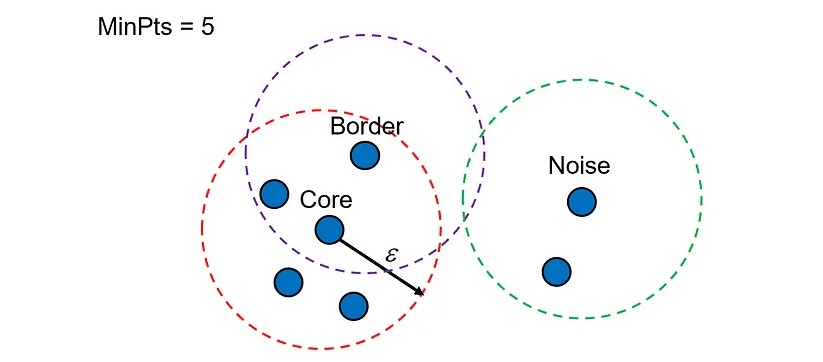
\includegraphics[scale = 0.5]{pic/figs/dbscanpoints.jpg}
        {\scriptsize Adopted from \href{https://ai.plainenglish.io/dbscan-density-based-clustering-aaebd76e2c8c}{ai.plainenglish.io}}
        \label{fig:dbscan-points}
    \end{figure}
\end{frame}


\begin{frame}{Core Concepts in DBSCAN (cont.)}
    
    \textbf{Definitions:}
    \begin{itemize}
        \item A point \( x_i \) is a core point if:
        \[
        |\{ x_j : d(x_i, x_j) \leq \epsilon \}| \geq \texttt{minPts}
        \]
        \item A point is a border point if it is within distance \( \epsilon \) of a core point, but not itself a core point.
    \end{itemize}
\end{frame}

\begin{frame}{DBSCAN Algorithm Steps}
    \textbf{Algorithm Steps:}
    \begin{enumerate}
        \item For each unvisited point $ x_i $:
        \begin{itemize}
            \item Mark $ x_i $ as visited.
            \item Find all points within distance $ \epsilon $ (neighborhood).
        \end{itemize}
        
        \item If $ x_i $ is a core point:
        \begin{itemize}
            \item Create a new cluster and expand it by recursively adding all reachable core and border points.
        \end{itemize}
        
        \item If $x_i$ is not a core point:
        \begin{itemize}
            \item Label it as noise if it does not belong to any cluster.
        \end{itemize}
    \end{enumerate}
\end{frame}

\begin{frame}{Advantages of DBSCAN}
    \begin{itemize}
        \item Can find clusters of arbitrary shape (non-spherical).
        \item Does not require specifying the number of clusters \( K \) in advance.
        \item Robust to noise and outliers.
        \item Works well with large datasets.
    \end{itemize}
    \begin{figure}
        \centering
        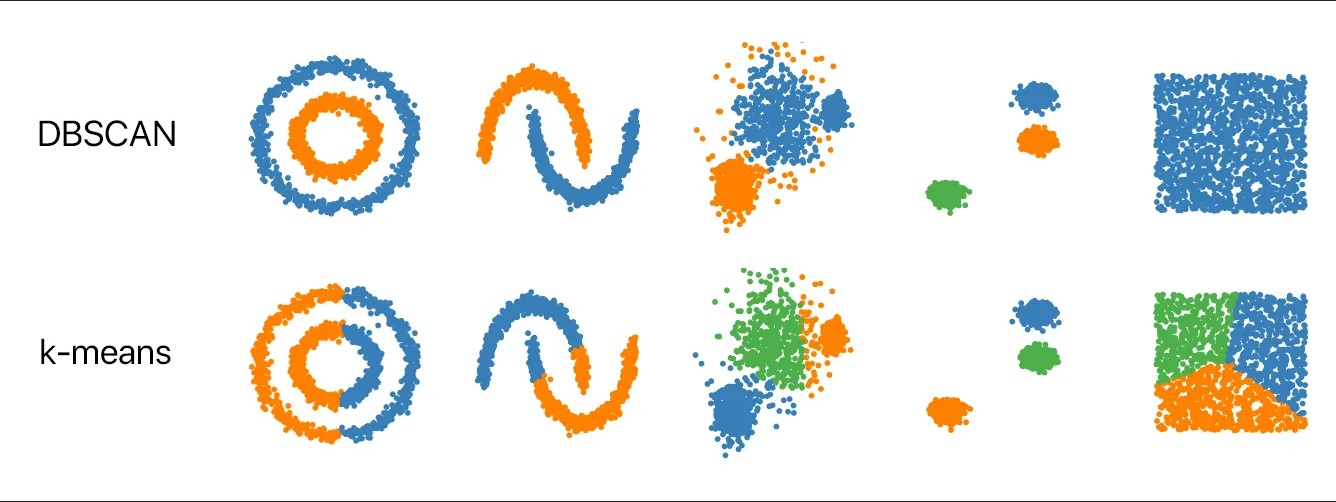
\includegraphics[scale = 0.45]{pic/figs/dbscan.jpg}
        {\scriptsize Adopted from \href{https://mrinalyadav7.medium.com/dbscan-algorithm-c894701306d5}{mrinalyadav7.medium.com}}
        \caption{DBSCAN vs K-Means.}
        \label{fig:dbscan-kmeans}
    \end{figure}
\end{frame}

\begin{frame}{Limitations of DBSCAN}
    \begin{itemize}
        \item DBSCAN struggles with datasets of varying densities.
        \item Sensitive to the selection of parameters $ \epsilon $ and \texttt{minPts}.
        \item Does not perform well with high-dimensional data.
    \end{itemize}
\end{frame}


\begin{frame}{Clustering Algorithms}
\begin{itemize}
 \item Each algorithm is suited for different kinds of patterns and information in data.
\end{itemize}
\begin{figure}
    \centering
    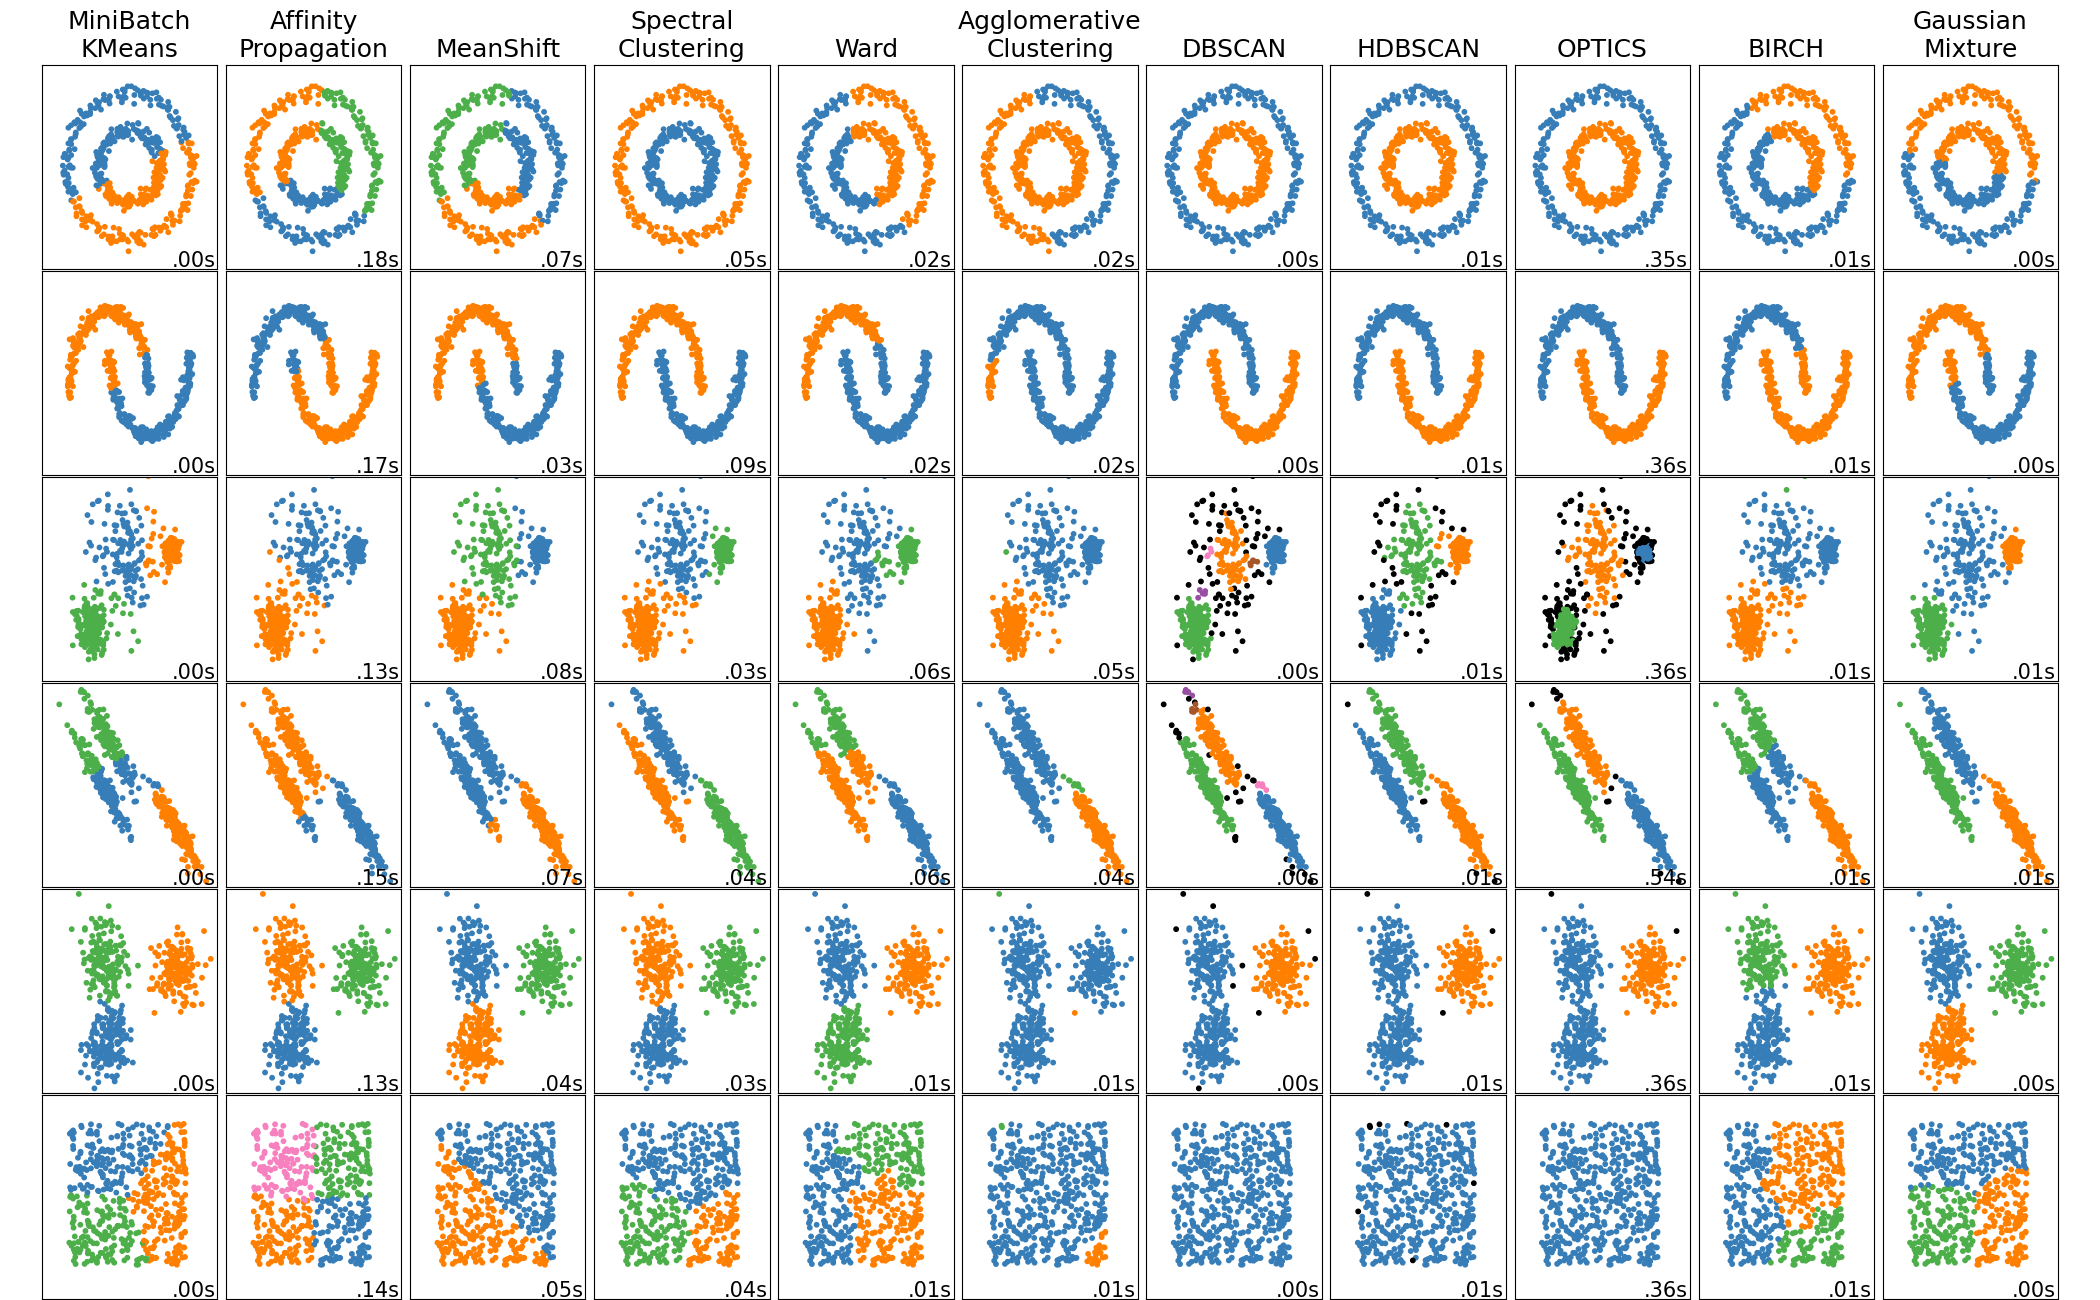
\includegraphics[width=\textwidth]{pic/figs/sphx_glr_plot_cluster_comparison_001.png}{\scriptsize Adopted from \href{https://scikit-learn.org/stable/auto_examples/cluster/plot_cluster_comparison.html}{scikit-learn.org}}
    \caption{clustering algorithms in action.}
    \label{fig:clustering algorithms}
\end{figure}
\end{frame}


% \begin{frame}{References}
%     \begin{itemize}
%         \item \cite{M2006-mk}
%         \item \cite{MITNeuroscienceLecture2014}
%         \item \cite{SontagMLLecture2012}
%         \item \cite{soleymaniMLCourse}
        
%     \end{itemize}
% \end{frame}

\begin{frame}{Contributions}
\begin{itemize}
\item \textbf{This slide has been prepared thanks to:}
\begin{itemize}
\item \href{https://hoomanzolfaghari84.github.io/}{Hooman Zolfaghari}
    % \setlength{\itemsep}{10pt} % Adjust the value to control the spacing
    % \item \href{https://github.com/Mahan-Bayhaghi}{Mahan Bayhaghi}
\end{itemize}
\end{itemize}

\end{frame}

\begin{frame}[allowframebreaks]
    \bibliography{ref}
    \bibliographystyle{ieeetr}
    \nocite{*}
\end{frame}

\end{document}